\documentclass{beamer}
\usepackage{amsmath}
\usepackage{amssymb}
\usepackage{pgf}
\usepackage{tikz}
\usepackage{listings}
\usepackage{color}
\usetikzlibrary{matrix}
\usetheme{boxes}
\newcommand{\fig}{./figures} % common figure path
\newcommand{\dbbslsh}{\textbackslash \textbackslash} % common figure path
\newenvironment{myblock}[3]{%
\definecolor{smtbx}{rgb}{0.64,0.76,0.68}
\setbeamercolor{block body}{#2}
\setbeamercolor{block title}{#3}
\begin{block}{#1}}{\end{block}}
\newcommand{\frnzplt}{FranzPlot }
\title[Curve e Sup. - Lab 4]{Curve e Superfici per il Design \\ Laboratorio 4: Rette e piani nello spazio}
\author[Prof.ssa Scotti]{Prof.ssa Anna Scotti}
%\institute[dimat]{Long Inst.}
\date{14 Maggio 2019}

\begin{document}
%\lstset{language=POV}
\begin{frame}
\maketitle
\end{frame}
\section{Introduzione}
\begin{frame}
\frametitle{Materiali}
Nella con i materiale di oggi troverete:
\begin{itemize}
\item Questa presentazione (\texttt{lab4.pdf})
\end{itemize}
Nella cartella `Franzplot\_DCS' troverete invece:
\begin{itemize}
\item Gli eseguibili per lanciare \frnzplt
\end{itemize}
\end{frame}
%\section{Matrici in POVRay}

\section{Esercizi}
\begin{frame}
\frametitle{Esercizio 1-i}
\begin{itemize}

\item Rappresentare con \frnzplt il piano $\alpha$, i vettori giacitura e la normale al piano.
\begin{displaymath}
\alpha:
\begin{cases}
u + v\\
u\\
u+2~v
\end{cases}
\;\;\; u,v \in \mathbb{R}
\end{displaymath}
\item Rappresentare con \frnzplt il piano $\beta$, i vettori giacitura e la normale al piano.
\begin{displaymath}
\beta:
\begin{cases}
u + v+2\\
u\\
u+2~v-1
\end{cases}
\;\;\; u,v \in \mathbb{R}
\end{displaymath}
\item
Determinare la retta perpendicolare al piano $\beta$ dell'esercizio 2 e passante per il punto $\mathbf{P}$:
\begin{displaymath}
\mathbf{P} = \begin{bmatrix} 1\\ 0\\-2 \end{bmatrix}
\end{displaymath}
\end{itemize}


\end{frame}
\begin{frame}
\frametitle{Esercizio  1 - ii}
\begin{columns}
\begin{column}{0.48\textwidth}
\begin{displaymath}
\mathbf{v}_1=
\begin{bmatrix}
1\\1\\1
\end{bmatrix}
\end{displaymath}
\begin{displaymath}
\mathbf{v}_1=
\begin{bmatrix}
1\\0\\2
\end{bmatrix}
\end{displaymath}
\end{column}
\begin{column}{0.48\textwidth}
\begin{displaymath}
\mathbf{n} =
\mbox{det}
\begin{bmatrix}
\mathbf{e}_1 & \mathbf{e}_2 & \mathbf{e}_3\\
1 & 1 & 1 \\
1 & 0 & 2
\end{bmatrix}
=
\begin{bmatrix}
2\\-1\\-1
\end{bmatrix}
\end{displaymath}
\end{column}
\end{columns}
\begin{itemize}
\item Il piano $\beta$ ha la stessa normale del piano $\alpha$ ma non passa dell'origine, ma \`e traslata del vettore $\mathbf{p}=[2,0,-1]^T$
\end{itemize}

\end{frame}
\begin{frame}
\frametitle{Esercizio 1 - iii}
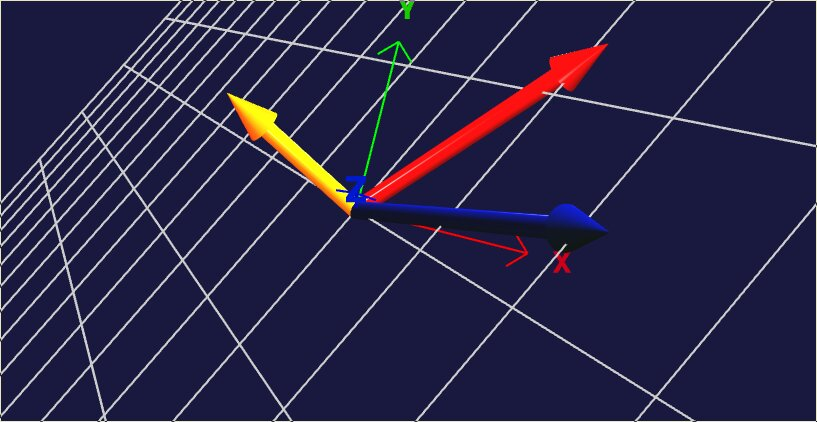
\includegraphics[width=0.9\textwidth]{\fig/l4_es1.jpeg}
\end{frame}

%
\begin{frame}[fragile]
\frametitle{Esercizio 1 - iv}
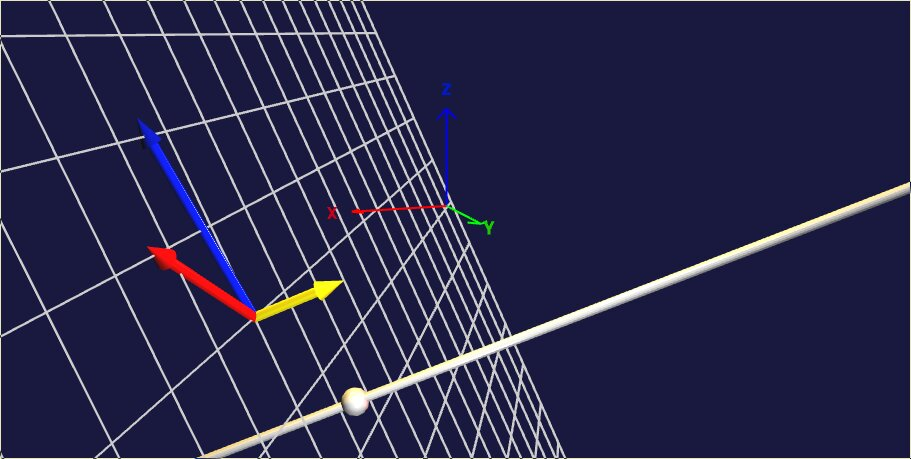
\includegraphics[width=0.9\textwidth]{\fig/l4_es1c.jpeg}

\end{frame}
%
%
\begin{frame}
\frametitle{Esercizio 2 - i}
\begin{itemize}
\item Rappresentare la retta $r$ passante per i punti
\begin{displaymath}
\mathbf{P}=\begin{bmatrix}2\\1\\1 \end{bmatrix},\;\;\;\;\;
\mathbf{Q}=\begin{bmatrix}1\\1\\3 \end{bmatrix};
\end{displaymath}
\item Determinare la retta $s$ perpendicolare ad $r$ e passante per:
\begin{displaymath}
\mathbf{M}=\begin{bmatrix}1\\2\\-2 \end{bmatrix}.
\end{displaymath}
\item Rappresentare il piano su cui giacciono i tre punti
\end{itemize}
\end{frame}
\begin{frame}
\frametitle{Esercizio 2 - ii}
\begin{columns}
\begin{column}{0.48\textwidth}
\begin{itemize}
\item Rappresentazione della retta $r$:
\end{itemize}
\end{column}
\begin{column}{0.48\textwidth}
\begin{displaymath}
r :\begin{cases} x = t +1\\ y = 1 \\z = -2~t+3 \end{cases}
\end{displaymath}
\end{column}
\end{columns}
\begin{columns}
\begin{column}{0.48\textwidth}
\begin{itemize}
\item Vettore che congiunge $\mathbf{M}$ ed un punto generico di $r$
\end{itemize}
\end{column}
\begin{column}{0.48\textwidth}
\begin{displaymath}
\mathbf{M} - r(t) = \begin{bmatrix} -t\\ 1 \\2t-5 \end{bmatrix}
\end{displaymath}
\end{column}
\end{columns}
\begin{columns}
\begin{column}{0.29\textwidth}
\begin{itemize}
\item Imponendo
\end{itemize}
\end{column}
\begin{column}{0.4\textwidth}
\begin{displaymath}
\begin{bmatrix} -t \\ 1 \\2t-5 \end{bmatrix}\cdot \begin{bmatrix}1\\ 0 \\-2 \end{bmatrix} = 0
\end{displaymath}
\end{column}
\begin{column}{0.29\textwidth}
trovo $t = 2$.
\end{column}
\end{columns}
\begin{columns}
\begin{column}{0.48\textwidth}
\begin{itemize}
\item Sostituisco nell'espressione per $s(t)$, trovando:
\end{itemize}
\end{column}
\begin{column}{0.48\textwidth}
\begin{displaymath}
s:
\begin{cases}
x  = -2t + 1 \\
y  =  t  + 2 \\
z  = -t  - 2
\end{cases}
\end{displaymath}
\end{column}
\end{columns}
\end{frame}
%
\begin{frame}
\frametitle{Esercizio 2 - iii}
Date le espressioni di $r$ ed $s$, una rappresentazione parametrica del piano \`e : 
\begin{displaymath}
\beta:\begin{cases}
x = -2u-v +3\\
y = u+1\\
z = -u+2v-1
\end{cases}
\end{displaymath}
Il vettore normale pu\`o calcolarsi come il prodotto vettoriale dei due vettori giacitura:

\begin{displaymath}
\mathbf{n} =
\mbox{det}
\begin{bmatrix}
\mathbf{e}_1 & \mathbf{e}_2 & \mathbf{e}_3\\
-2 & 1 & -1 \\
-1 & 0 & 2
\end{bmatrix}
=
\begin{bmatrix}
2\\5\\1
\end{bmatrix}
\end{displaymath}
\end{frame}
%
\begin{frame}
\frametitle{Esercizio 2 - iv}
\begin{center}
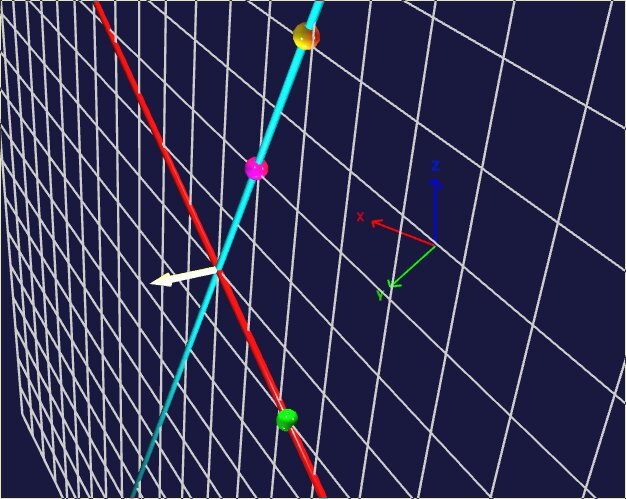
\includegraphics[width = 0.9\textwidth]{\fig/l4_es2.jpeg}
\end{center}
\end{frame}
%
\begin{frame}
\frametitle{Esercizio 3 - i}
Con \frnzplt \`e possibile rappresentare un piano parametricamente, come una superficie qualsiasi.
\begin{itemize}
\item Rappresentare la retta $r$:
\begin{displaymath}
r:\begin{cases}
x = t \\
y = 0.5~t\\
z = 0
\end{cases}
\end{displaymath}
\item Rappresentare l'oggetto che si ottiene: 
\begin{enumerate}
\item Traslando la retta in direzione $y$ facendo variare il parametro della traslazione tra -5 e 5.
\item Ruotanto rispetto a z la retta di $2\pi$ radianti.
\end{enumerate}
\end{itemize}
\end{frame}
\begin{frame}
\frametitle{Esercizio 3 - ii}
\begin{center}
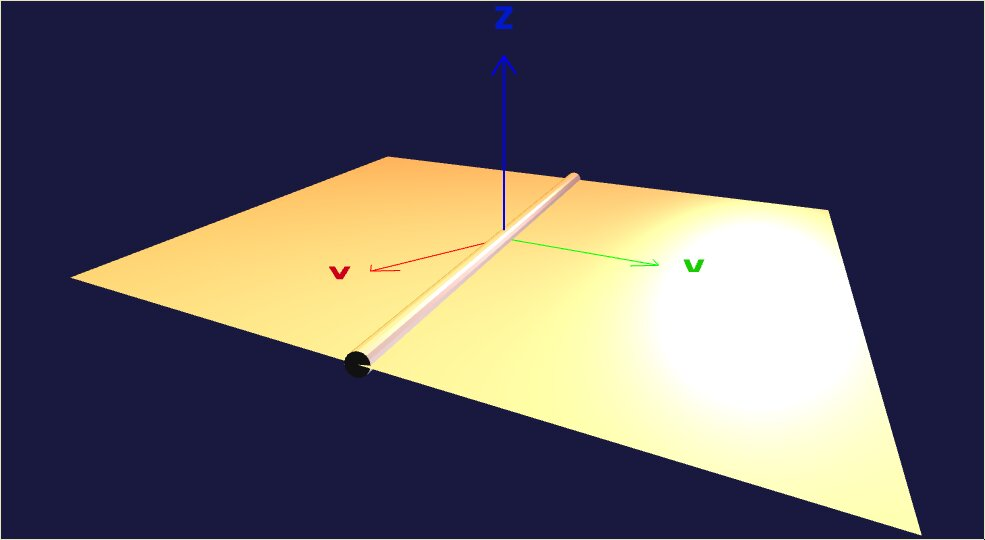
\includegraphics[width=0.5\textwidth]{\fig/l4_es3a.jpeg}
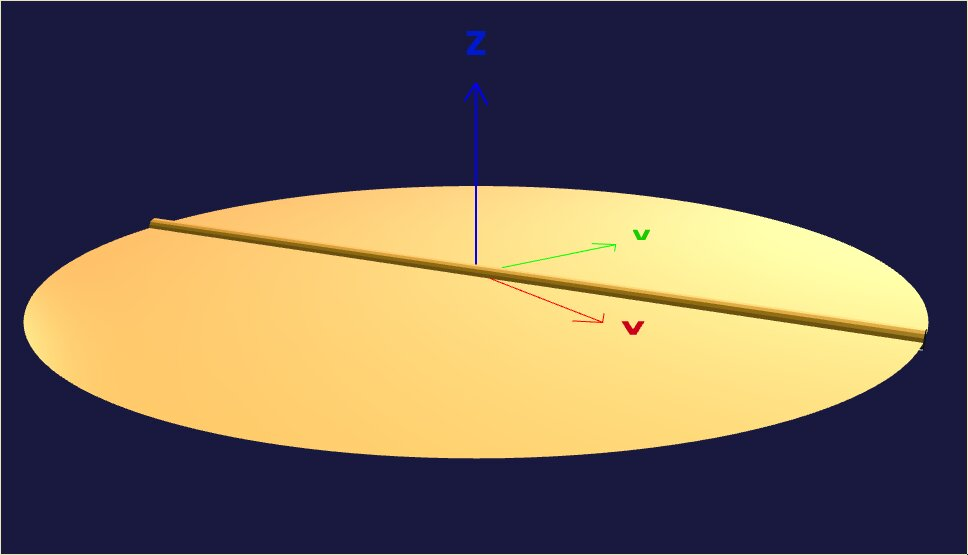
\includegraphics[width=0.5\textwidth]{\fig/l4_es3b.jpeg}
\end{center}
\end{frame}
\begin{frame}
\frametitle{Esercizio 4 - i}
Date le rette:
\begin{columns}

\begin{column}{0.33\textwidth}
\begin{displaymath}
p:\begin{cases} 
x = 3~t - \frac{1}{2}\\
y = t - \frac{1}{2}\\
z = -2~t
\end{cases}
\end{displaymath}
\end{column}
\begin{column}{0.33\textwidth}
\begin{displaymath}
q:\begin{cases} 
x = t - 13 \\
y = 2\\
z = -t + 15
\end{cases}
\end{displaymath}
\end{column}
\begin{column}{0.33\textwidth}
\begin{displaymath}
r:\begin{cases} 
x = t + \frac{3}{2}\\
y = t + \frac{1}{2}\\
z = 2~t -2
\end{cases}
\end{displaymath}
\end{column}
\end{columns}
\begin{itemize}
\item Rappresentare le rette con \frnzplt
\item Le rette $p$ e $q$ sono perpendicolari? E le rette $p$ ed $r$?
\item Determinare e rappresentare i punti di intersezione se presenti
\end{itemize}
\end{frame}
\begin{frame}
\frametitle{Esercizio 4 - ii}
\begin{itemize}
\item Scrivere l'equazione del piano $\alpha$ con normale $\mathbf{n}=[1,1,1]^T$ passante per il punto $(1,0,0)$. Rappresentare il piano con \frnzplt
\item Calcolare  e rappresentare i punti di intersezione di $p$ e $q$ con il piano.
\item Calcolare e rappresentare il piano $\beta$ su cui giacciono  le rette $p$ e $q$, e  scrivere l'espressione parametrica della retta $s$ intersezione dei piani $\alpha$ e $\beta$ 
\end{itemize}
\end{frame}
\begin{frame}
\frametitle{Esercizio 4 - iii}
\begin{center}
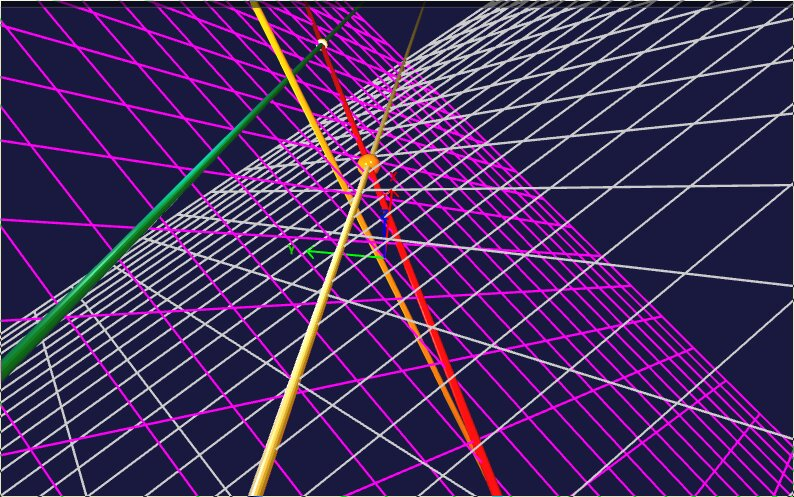
\includegraphics[width=0.9\textwidth]{\fig/l4_es5final.jpeg}
\end{center}
\end{frame}

\end{document}
